\section{Lessons Learned}
\label{sec:lessons-learned}

The Peg Solitaire game is a fascinating puzzle that not only provides entertainment but also serves as an excellent exercise in problem-solving and algorithm design. Through the process of developing a solution for this game, I have learned several valuable lessons that extend beyond the confines of this specific project.

\subsection{Project Management}
Developing the Peg Solitaire game provided valuable lessons in project management and software development practices:

\subsubsection{Incremental Development}
I adopted an incremental development approach, focusing on one feature at a time. The project's evolution can be traced through the incremental prompts found in the \texttt{/prompts} directory, which document the step-by-step progression:

\begin{itemize}
    \item Starting with a basic game structure and homepage (01-init.md)
    \item Adding game mode selection (02-start.md)
    \item Implementing settings functionality (03-settings.md)
    \item Creating various game boards (04-gamemodes.md)
    \item Developing the UI elements (05-buttonUI.md, 06-gameUI.md)
    \item Adding core gameplay features (07-winandlose.md, 08-keyboard.md, 09-selection.md)
    \item Implementing special modes (10-anti.md)
    \item Adding advanced features like strategy suggestions (11-strategy.md)
    \item Enhancing the user experience (12-information.md)
    \item Optimizing algorithms (13-optimize.md)
    \item Creating the loading animation (14-loading.md)
    \item Developing the endgame mode (15-endgame.md)
\end{itemize}

This approach allowed for continuous progress and clear direction, ensuring that each component functioned properly before moving on to the next.

\subsubsection{Modular Architecture}
Implementing the Model-View-Controller (MVC) pattern was crucial for maintaining code organization and facilitating feature additions:

\begin{itemize}
    \item \textbf{Model}: The \texttt{Board} class encapsulates the game state and rules, independent of the user interface
    \item \textbf{View}: Classes like \texttt{BoardView} and \texttt{GameView} handle visual representation and user input
    \item \textbf{Controller}: The \texttt{BoardController} class mediates between the model and view, processing user actions and updating the game state
\end{itemize}

This separation of concerns made it easier to:
\begin{itemize}
    \item Add new features without breaking existing functionality
    \item Test components in isolation
    \item Maintain a clean and understandable codebase
\end{itemize}

\subsubsection{Version Control and Documentation}
The project benefited from proper version control practices and thorough documentation:

\begin{itemize}
    \item Git was used for tracking changes and managing development
    \item Commit messages provided clear explanations of implementation choices
    \item Code comments and documentation made the codebase more accessible
    \item A comprehensive README file provided build instructions and feature overviews
\end{itemize}

\subsection{Algorithm Design}
The development of this project provided significant insights into algorithm design and optimization techniques:

\subsubsection{Recursive Backtracking}
Implementing the solution-finding algorithm for Peg Solitaire offered valuable lessons in recursive algorithms:

\begin{itemize}
    \item The depth-first search approach proved effective for exploring possible move sequences
    \item Proper backtracking ensured all potential solutions were considered
    \item Base cases needed careful consideration to prevent infinite recursion
    \item The practical limitations of pure recursion became evident as the search space grew exponentially
\end{itemize}

\subsubsection{Optimization Techniques}
Facing performance challenges with the naive implementation led to learning several important optimization strategies:

\begin{itemize}
    \item \textbf{Pattern Recognition}: Identifying board symmetries reduced the search space significantly. The recognition that rotating or flipping the board produces equivalent game states led to a major algorithmic improvement.
   
    \item \textbf{Memoization}: Caching previously computed results avoided redundant calculations. The static cache of unsolvable board states dramatically improved performance:

    \item \textbf{Bit Manipulation}: Using bit operations to create compact board state representations improved memory efficiency and comparison speed
\end{itemize}

\subsubsection{Multithreading}
Implementing the strategy calculation worker thread taught important principles of concurrent programming:

\begin{itemize}
    \item Separating CPU-intensive tasks from the UI thread maintained application responsiveness
    \item Proper synchronization mechanisms (mutexes, signals/slots) prevented race conditions
    \item Cancellation mechanisms allowed for interrupting long-running operations when the board state changed
    \item Thread-safe data structures ensured consistent state across threads
\end{itemize}

\subsubsection{Generative Algorithms}
The Endgame mode required a novel approach to generating random but solvable puzzles:

\begin{itemize}
    \item Working backward from the winning state guaranteed solvability
    \item Applying random ``reverse moves" created diverse puzzle configurations
    \item This reverse-engineering approach ensured the generated puzzles were both challenging and fair
\end{itemize}

\subsection{Understanding of the C++ Language}
This project significantly deepened my understanding of modern C++ and object-oriented programming principles:

\subsubsection{Object-Oriented Design}
Working with C++ reinforced key OOP concepts:

\begin{itemize}
    \item \textbf{Encapsulation}: Properly hiding implementation details behind public interfaces improved maintainability. For example, the \texttt{Board} class encapsulates all board state management:
    \begin{center}
        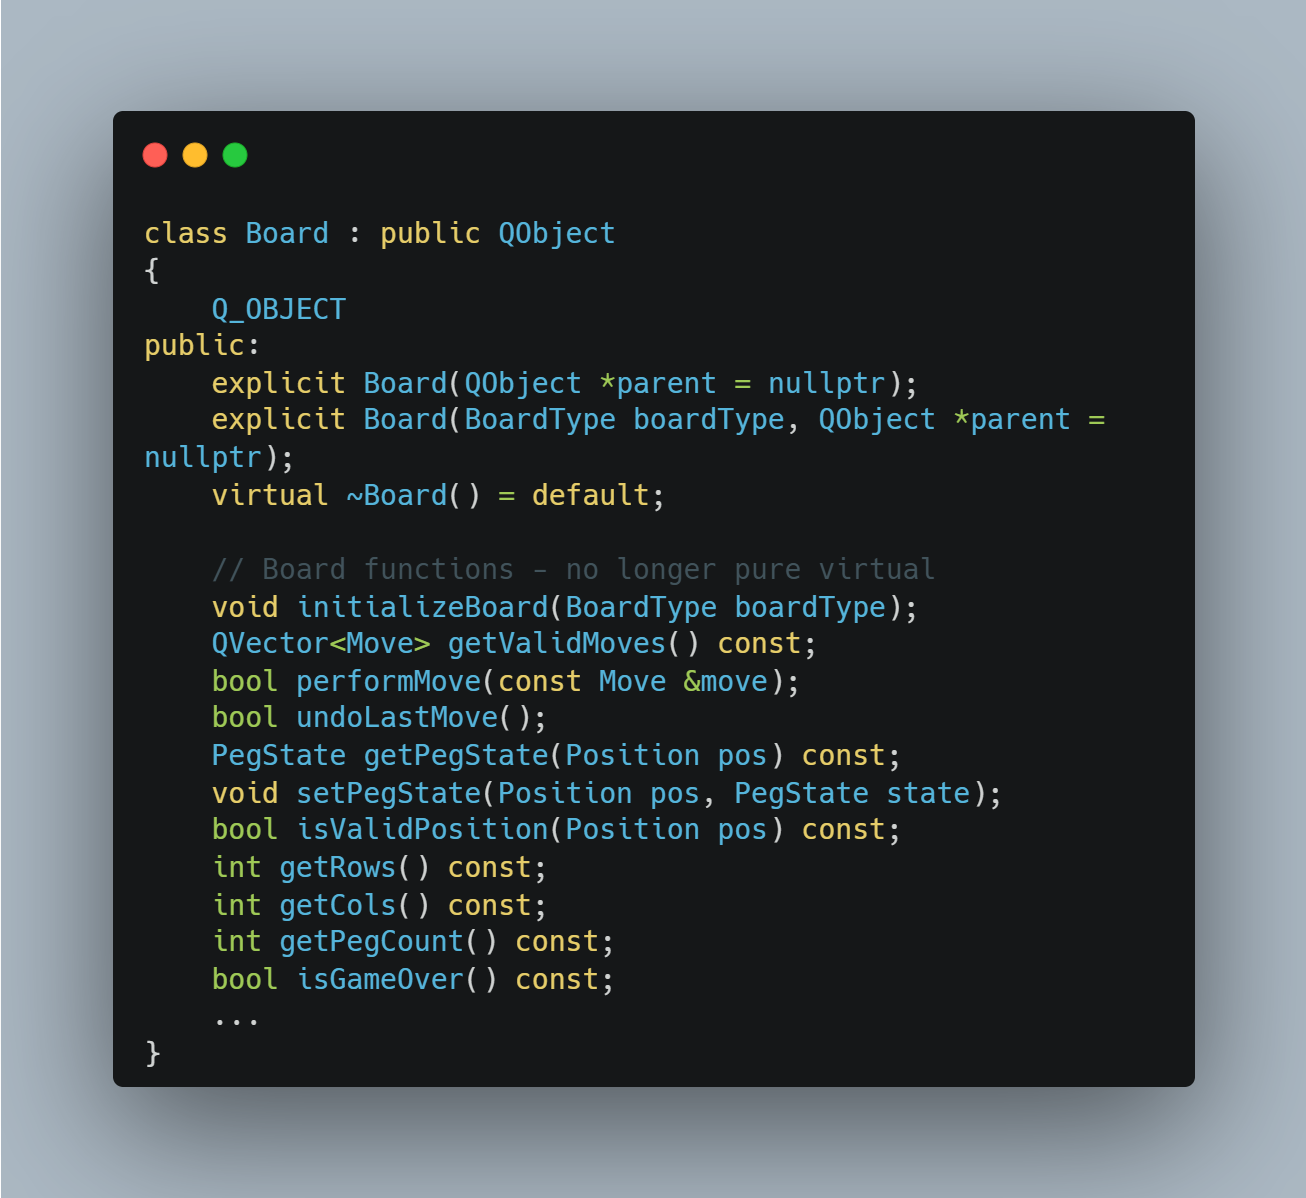
\includegraphics[width=0.6\textwidth]{resource/code-examples/BoardDeclaration.png}
    \end{center}
    \item \textbf{Inheritance}: Extending Qt classes allowed for customizing behavior while leveraging existing functionality
    \item \textbf{Polymorphism}: Using virtual functions and overriding methods like \texttt{paintEvent} in UI components
    \item \textbf{Composition}: Building complex objects from simpler ones, such as composing the game view from multiple UI elements
\end{itemize}

\subsubsection{Modern C++ Features}
The project provided opportunities to utilize modern C++ features:

\begin{itemize}
    \item \textbf{Strong Typing}: Using enum classes for type-safe enumerations (\texttt{BoardType}, \texttt{PegState})
    \item \textbf{Auto Type Deduction}: Simplifying code with automatic type inference where appropriate
    \item \textbf{Smart Pointers}: Managing object lifetimes, although Qt's parent-child relationship system was primarily used
    \item \textbf{Lambda Expressions}: Implementing concise callbacks for event handling and signal connections
    \item \textbf{Range-based Loops}: Writing cleaner iteration code for collections
\end{itemize}

\subsubsection{Qt Framework Integration}
Working with the Qt framework enhanced my understanding of:

\begin{itemize}
    \item \textbf{Signal-Slot Mechanism}: Implementing loosely coupled communication between components
    \item \textbf{Meta-Object System}: Leveraging Qt's reflection capabilities with the Q\_OBJECT macro
    \item \textbf{Event Handling}: Overriding event methods to handle mouse, keyboard, and paint events
    \item \textbf{Custom Painting}: Implementing custom drawing routines with QPainter for the board visualization
    \item \textbf{Layouts}: Creating responsive UIs that adapt to window resizing
    \item \textbf{Widget Management}: Creating, organizing, and managing hierarchical UI components
\end{itemize}

\subsubsection{Memory Management}
The project highlighted important aspects of memory management in C++:

\begin{itemize}
    \item Understanding object ownership models in Qt's parent-child relationship system
    \item Properly cleaning up resources when objects are no longer needed
    \item Avoiding memory leaks by ensuring proper object destruction
    \item Managing dynamically allocated memory for temporary objects (like test boards in the solving algorithm)
\end{itemize}

\subsubsection{Performance Considerations}
Writing performance-critical code provided insights into C++ optimization:

\begin{itemize}
    \item Using pass-by-reference for large objects to avoid expensive copying
    \item Employing const correctness to communicate intent and enable compiler optimizations
    \item Understanding when to use different container types based on access patterns
    \item Minimizing object creation and destruction in tight loops
    \item Profiling and identifying bottlenecks in the algorithm implementation
\end{itemize}